\documentclass[border=10pt]{standalone}
\usepackage{pgfplots}
\usepgfplotslibrary{fillbetween}
\pgfplotsset{compat=1.18}
\begin{document}
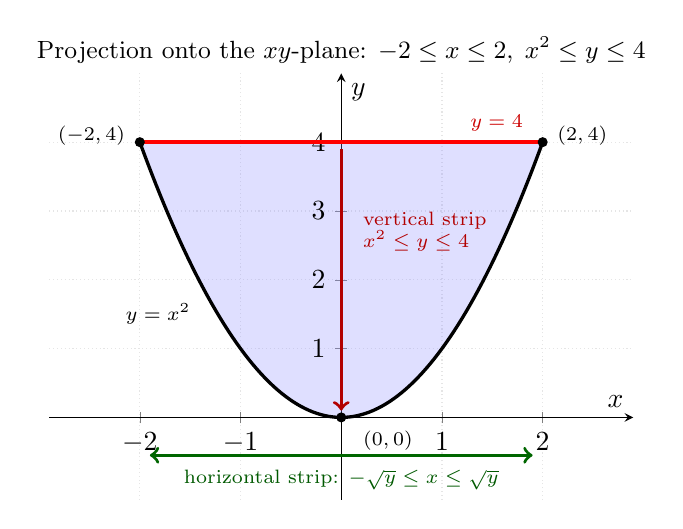
\begin{tikzpicture}
\begin{axis}[width=9cm, height=7cm, axis lines=middle,
    xlabel={$x$}, ylabel={$y$}, xmin=-2.9,xmax=2.9, ymin=-1.2,ymax=5.0,
    xtick={-2,-1,1,2}, ytick={1,2,3,4},
    grid=major, grid style={gray!20,densely dotted}]
  \addplot[name path=PAR, blue!45, opacity=0, domain=-2:2, samples=101] {x^2};
  \addplot[name path=TOP, blue!45, opacity=0, domain=-2:2, samples=2] {4};
  \addplot[fill=blue!45, opacity=0.28] fill between[of=PAR and TOP];
  \addplot[very thick, domain=-2:2, samples=101] {x^2};
  \node[font=\scriptsize, anchor=east] at (axis cs:-1.4,1.5) {$y=x^2$};
  \addplot[red, very thick, domain=-2:2, samples=2] {4};
  \node[font=\scriptsize, anchor=south east, text=red!80!black] at (axis cs:1.9,4.02) {$y=4$};
  \draw[->, red!70!black, very thick] (0,3.9) -- (0,0.1);
  \node[font=\scriptsize, text=red!70!black, align=left, anchor=west] at (axis cs:0.12,2.7) {vertical strip\\ $x^2\le y\le 4$};
  \draw[<->, green!40!black, very thick] (-1.9,-0.55) -- (1.9,-0.55);
  \node[font=\scriptsize, text=green!35!black, align=center, anchor=north] at (axis cs:0,-0.62) {horizontal strip: $-\sqrt{y}\le x\le\sqrt{y}$};
  \addplot[only marks, mark=*, mark size=1.6] coordinates {(-2,4) (2,4) (0,0)};
  \node[font=\scriptsize, anchor=east]  at (axis cs:-2.05,4.1) {$(-2,4)$};
  \node[font=\scriptsize, anchor=west]  at (axis cs: 2.05,4.1) {$(2,4)$};
  \node[font=\scriptsize, anchor=north west] at (axis cs:0.12,-0.05) {$(0,0)$};
\end{axis}
\node[font=\small, align=center, anchor=south] at (current bounding box.north) {Projection onto the $xy$-plane:  $-2\le x\le 2,\;x^2\le y\le 4$};
\end{tikzpicture}
\end{document}
